\documentclass[12pt]{article}
\usepackage{polski}
\usepackage[utf8]{inputenc}
\usepackage{graphicx}
\usepackage{amsmath}
\usepackage{graphicx}
\usepackage{setspace}
\usepackage{pdfpages}
\onehalfspacing


\title{ Badanie temperaturowej zależności współczynnika 
    lepkości cieczy metodą wiskozymetru Höpplera \\
    \large Informatyka – profil praktyczny, semestr II \\
    Wydział Matematyki Stosowanej \\
    Politechnika Śląska \\}

\author{ Sekcja 5 \\
    Piotr Skowroński}
\date{Kwiecień 2022}

\begin{document}

\maketitle

\section{Wstęp teoretyczny.}
Każde ciało poruszające się w cieczy czy gazie doznaje
siłę oporu, z powodu tego, że warstwy cieczy przylegającej do ciała
będącego w ruchu pociągają za sobą coraz dalsze warstwy sąsiednie.
Mamy tu do czynienia z przesuwaniem się jednych warstw cieczy względem
drugich, co powoduje tarcie wewnętrzne, które spowalnia ruch cząstek i ciała.
Ta siła oporu zależna jest od lepkości cieczy, a lepkość cieczy zależna
jest od rodzaju cieczy, a co ważniejsze, od temperatury. Ruchy termiczne 
cząsteczek mają wpływ na siły oddziaływania międzycząsteczkowego. 
W cieczach wzrost prędkości ruchów termicznych siły te osłabia (lepkość maleje),
w gazach sytuacja jest odwrotna.

Współczynnik lepkości cieczy można wyznaczyć przez wyznaczenie średniego czasu 
spadania kulki w cieczy.

Celem wykonywanego ćwiczenia jest  wyznaczenie zależności współczynnika 
lepkości cieczy od temperatury metodą wiskozymetru Höpplera. Doświadczenie 
polega na mierzeniu czasu opadania kulki dla zmieniających się temperatur cieczy.
\section{Pomiary}

Podczas wykonywania doświadczenia w pracowni pomiary zapisywałem ręcznie na
kartce. Następnie przepisałem wyniki moich pomiarow do pliku CSV, by
umożliwić ich wykorzystanie w programie.

Użyłem języka Python w środowisku Jupyter Notebook. Wykorzystałem biblioteki
\textit{numpy} oraz \textit{matplotlib}.

\section{Obliczenia i wykresy}

\subsection*{Obliczenie niepewności typu $a$ (statystycznych) średnich czasów spadania $u_a(t_{sr})$.}

Aby policzyć niepewności typu $a$ skorzystamy ze wzoru:
\begin{center}
    $u_a(t_{sr}) = \sqrt{\frac{1}{N(N-1)} \displaystyle\sum_{i=1}^{N} (t_i - t_{sr})^2} \cdot t_{\alpha, N}$.
\end{center}
Gdzie:
\begin{flushleft}
    $t_{\alpha, N}$ - Współczynnik Studenta Fishera, gdzie za $\alpha$ przyjmujemy 0.6828, a za $N$
    liczbę pomiarów w serii, czyli w naszym przypadku 2.
\end{flushleft}
\begin{center}
    $t_{\alpha=0.6828,N=5} = 1.141$.
\end{center}
Tabelka niepewności statystycznych:
\begin{center}
    \begin{tabular}{ | c | c | c | }
        \hline
        Lp. & $t_{sr}$, s & $u_a(t_{sr})$, s \\ \hline
        1.  & 171.0    & 2.5           \\ \hline
        2.  & 133.0    & 2.4           \\ \hline
        3.  & 102.0    & 2.9           \\ \hline
        4.  & 87.9     & 2.5           \\ \hline
        5.  & 77.2     & 2.2           \\ \hline
        6.  & 63.7     & 2.4           \\ \hline
    \end{tabular}
\end{center}
\subsection*{Obliczenie całkowitej niepewności czasów $u(t_{sr})$.}
Aby policzyć niepewności całkowite czasów spadania $u(t_{sr})$
skorzystamy ze wzoru:
\begin{center}
    $u(t_{sr}) = \sqrt{u_a^2(t_{sr}) + u_b^2(t_{sr})}$.
\end{center}
Gdzie za $u_b(t_{sr})$ przyjmuje niepewność czasu reakcji
człowieka $u_b(t_{sr})$=0.3 s

\subsection*{Obliczenie współczynnika lepkości oleju
    parafinowego $\eta$ dla każdej temperatury $T$.}

Do policzenia współczynnika lepkości $\eta$ skorzystam
ze wzoru:
\begin{center}
    $\eta = K(\rho_k - \rho)t$.
\end{center}
Gdzie: \\
\indent $K=1.2018 \cdot 10^{-6} \frac{m^2}{s^2}$ - stała aparaturowa. \\
\indent $\rho_k = 8150 \frac{kg}{m^3}$ - gęstość stalowej kulki. \\
\indent $\rho$ - gęstość oleju parafinowego w różnych temperaturach.

\subsection*{Obliczenie niepewności współczynnika lepkości
    $\eta$ \\
    korzystając z prawa przenoszenia niepewności.}

Wzór na prawo przenoszenia niepewności ma postać:
\begin{center}
    $u(y) = \sqrt{\sum_{i=1}^{k}[\frac{\partial y}{\partial x_i}u(x_i)]^2}$
\end{center}
Zatem prawo przenoszenia niepewności dla $\eta$ ma postać:
\begin{center}
    $u(\eta) = \sqrt{ [K(\rho_k - \rho)u(t)]^2 } = K(\rho_k - \rho)u(t)$.
\end{center}
Tabelka z danymi:
\begin{center}
    \begin{tabular}{ | c | c | c | c | c | c | }
        \hline
        Lp. & T, $^{\circ}$C & $t_{sr}$, s & $u(t_{sr})$, s & $\eta$, Pa$\cdot$s & $u(\eta)$, Pa$\cdot$s \\ \hline
        1.  & 21.0           & 171.0       & 2.5            & 1.500              & 0.022                 \\ \hline
        2.  & 26.5           & 133.0       & 2.4            & 1.160              & 0.021                 \\ \hline
        3.  & 31.0           & 103.0       & 2.9            & 0.897              & 0.026                 \\ \hline
        4.  & 34.0           & 87.9        & 2.5            & 0.769              & 0.022                 \\ \hline
        5.  & 36.0           & 77.2        & 2.2            & 0.676              & 0.019                 \\ \hline
        6.  & 40.5           & 63.7        & 2.5            & 0.557              & 0.022                 \\ \hline
    \end{tabular}
\end{center}

\subsection*{Wykres zależności współczynnika lepkości $\eta$ od \\
    temperatury $T$ i wykres zależności logarytmu \\
    naturalnego współczynnika lepkości $\ln(\eta)$ od \\
    odwrotności temperatury $\frac{1}{T}$.}

Za niepewność temperatury $u(T)$ przyjmujemy $0.5^{\circ}C$ związane
z niedokładnym odczytem temperatury na termometrze. \\ 
Wykresy na następnych stronach:
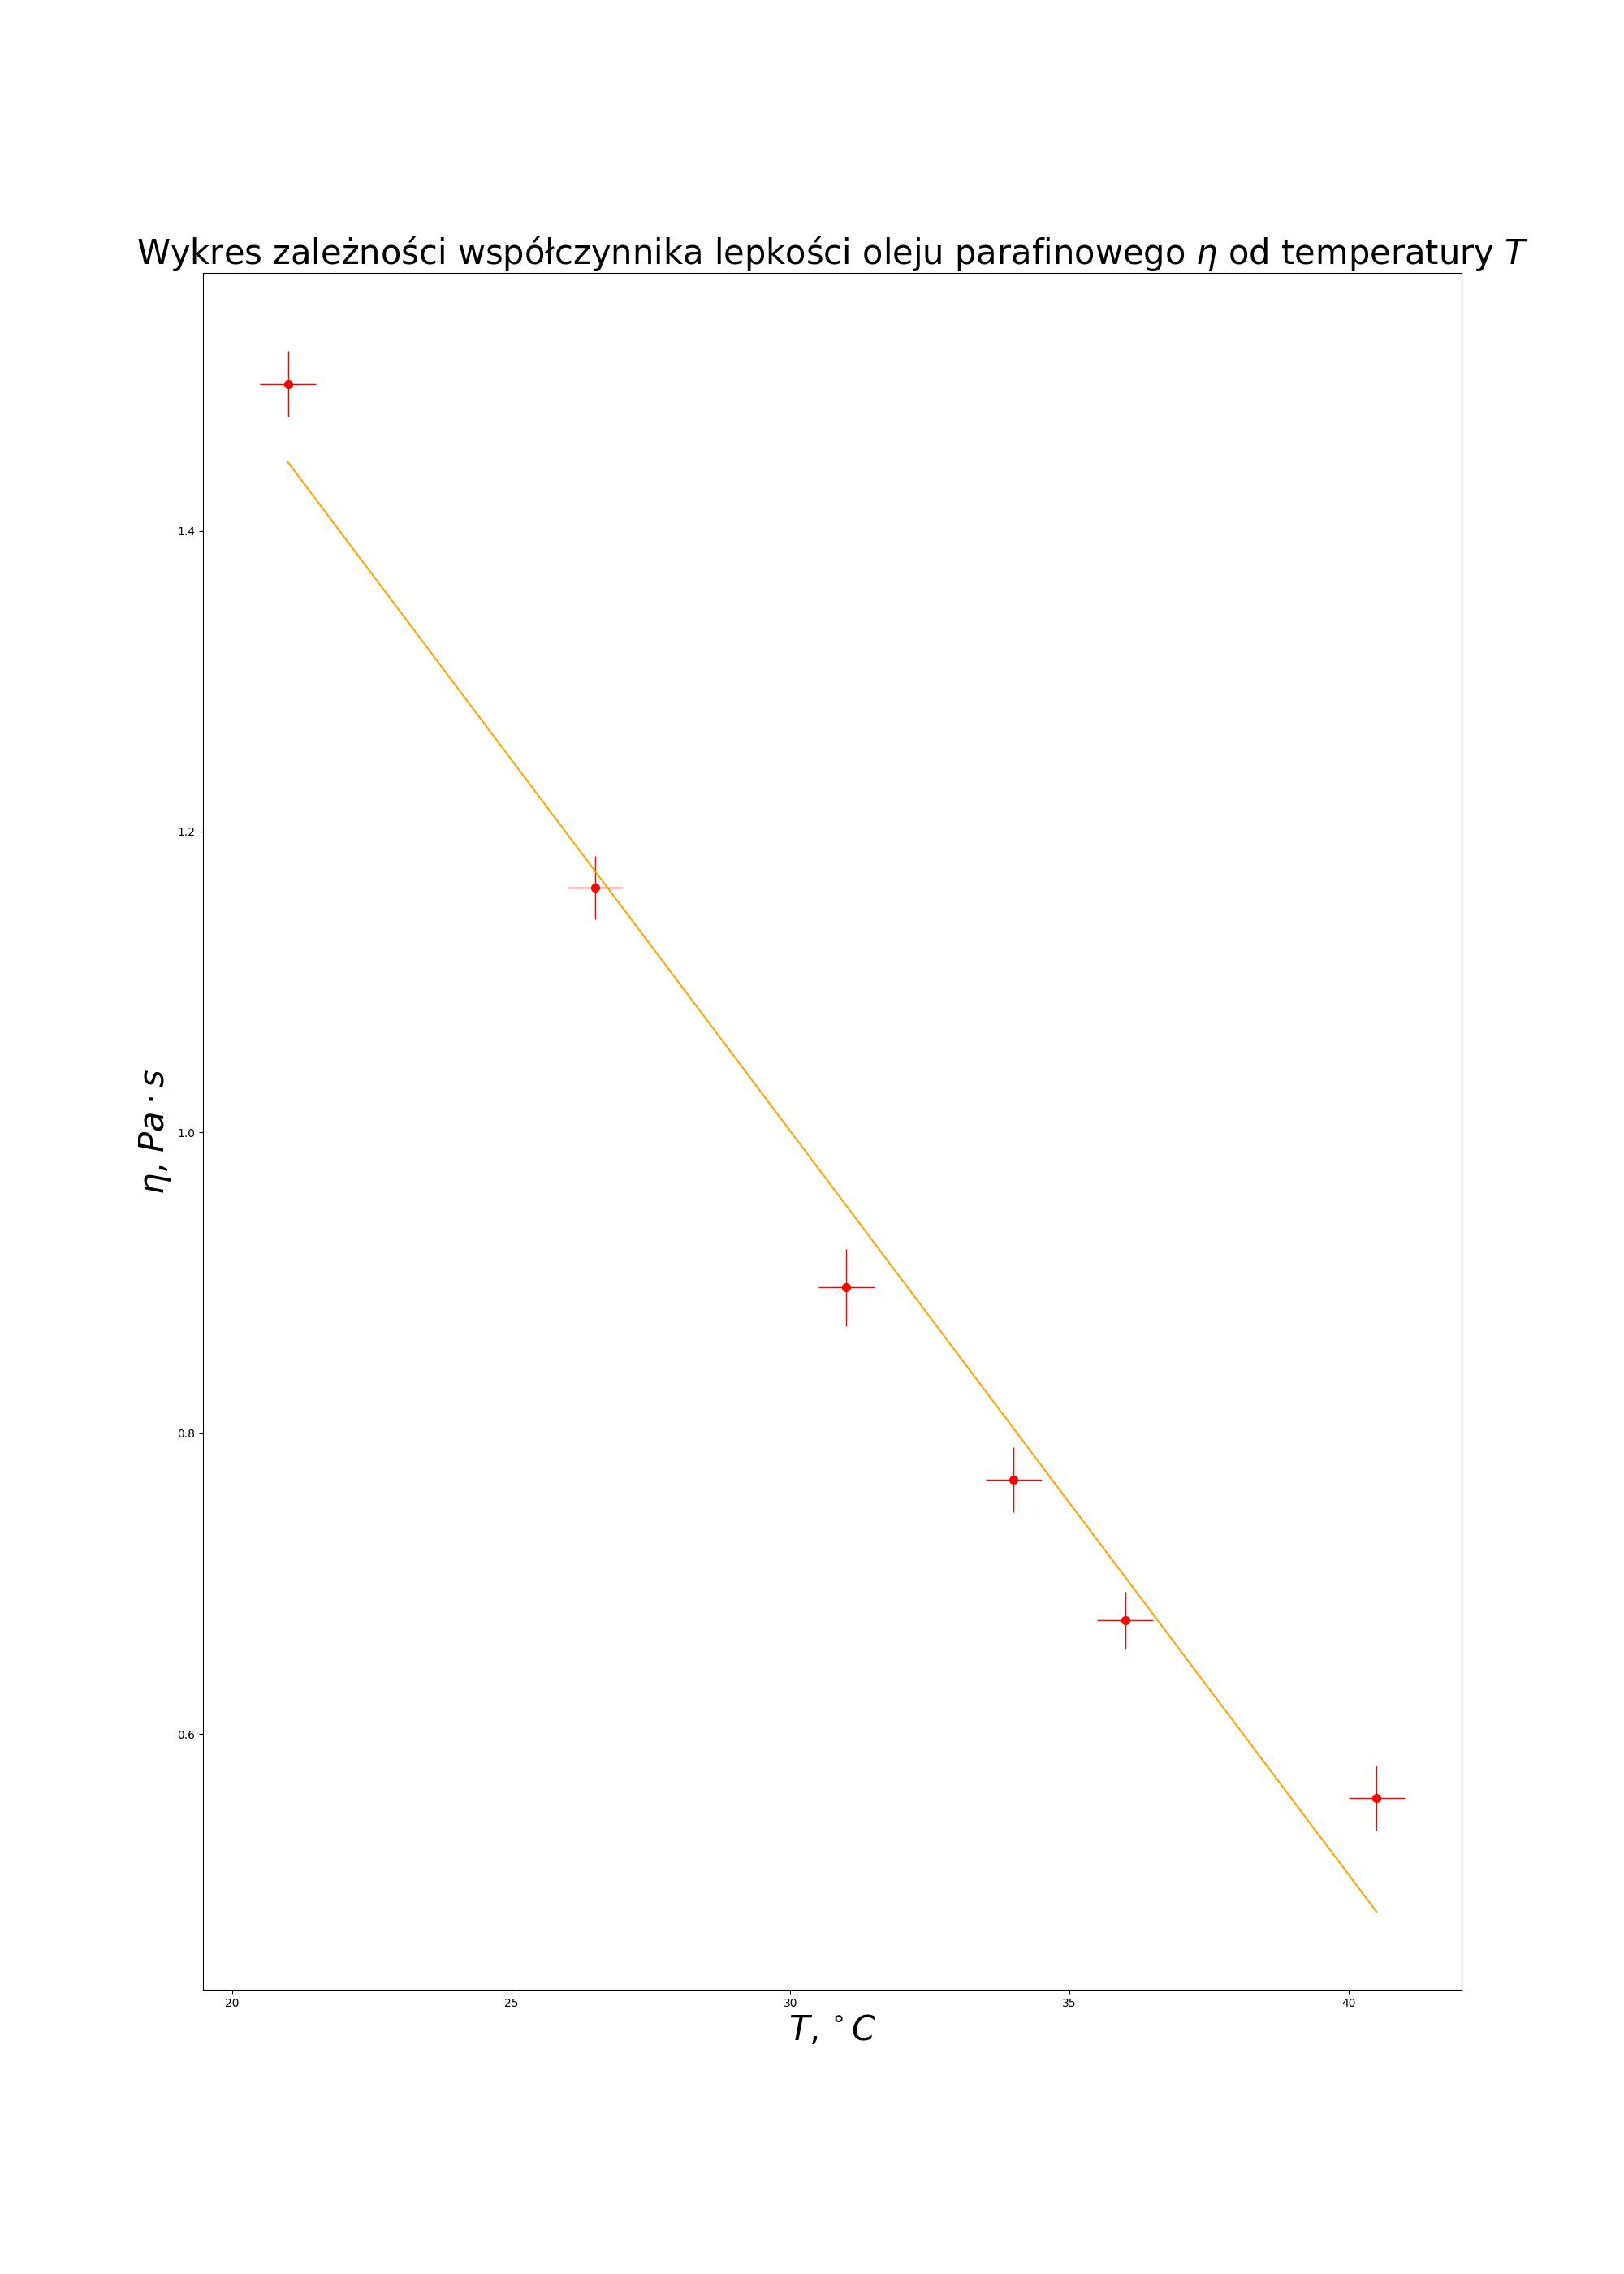
\includepdf{./img/wykres1.jpg}
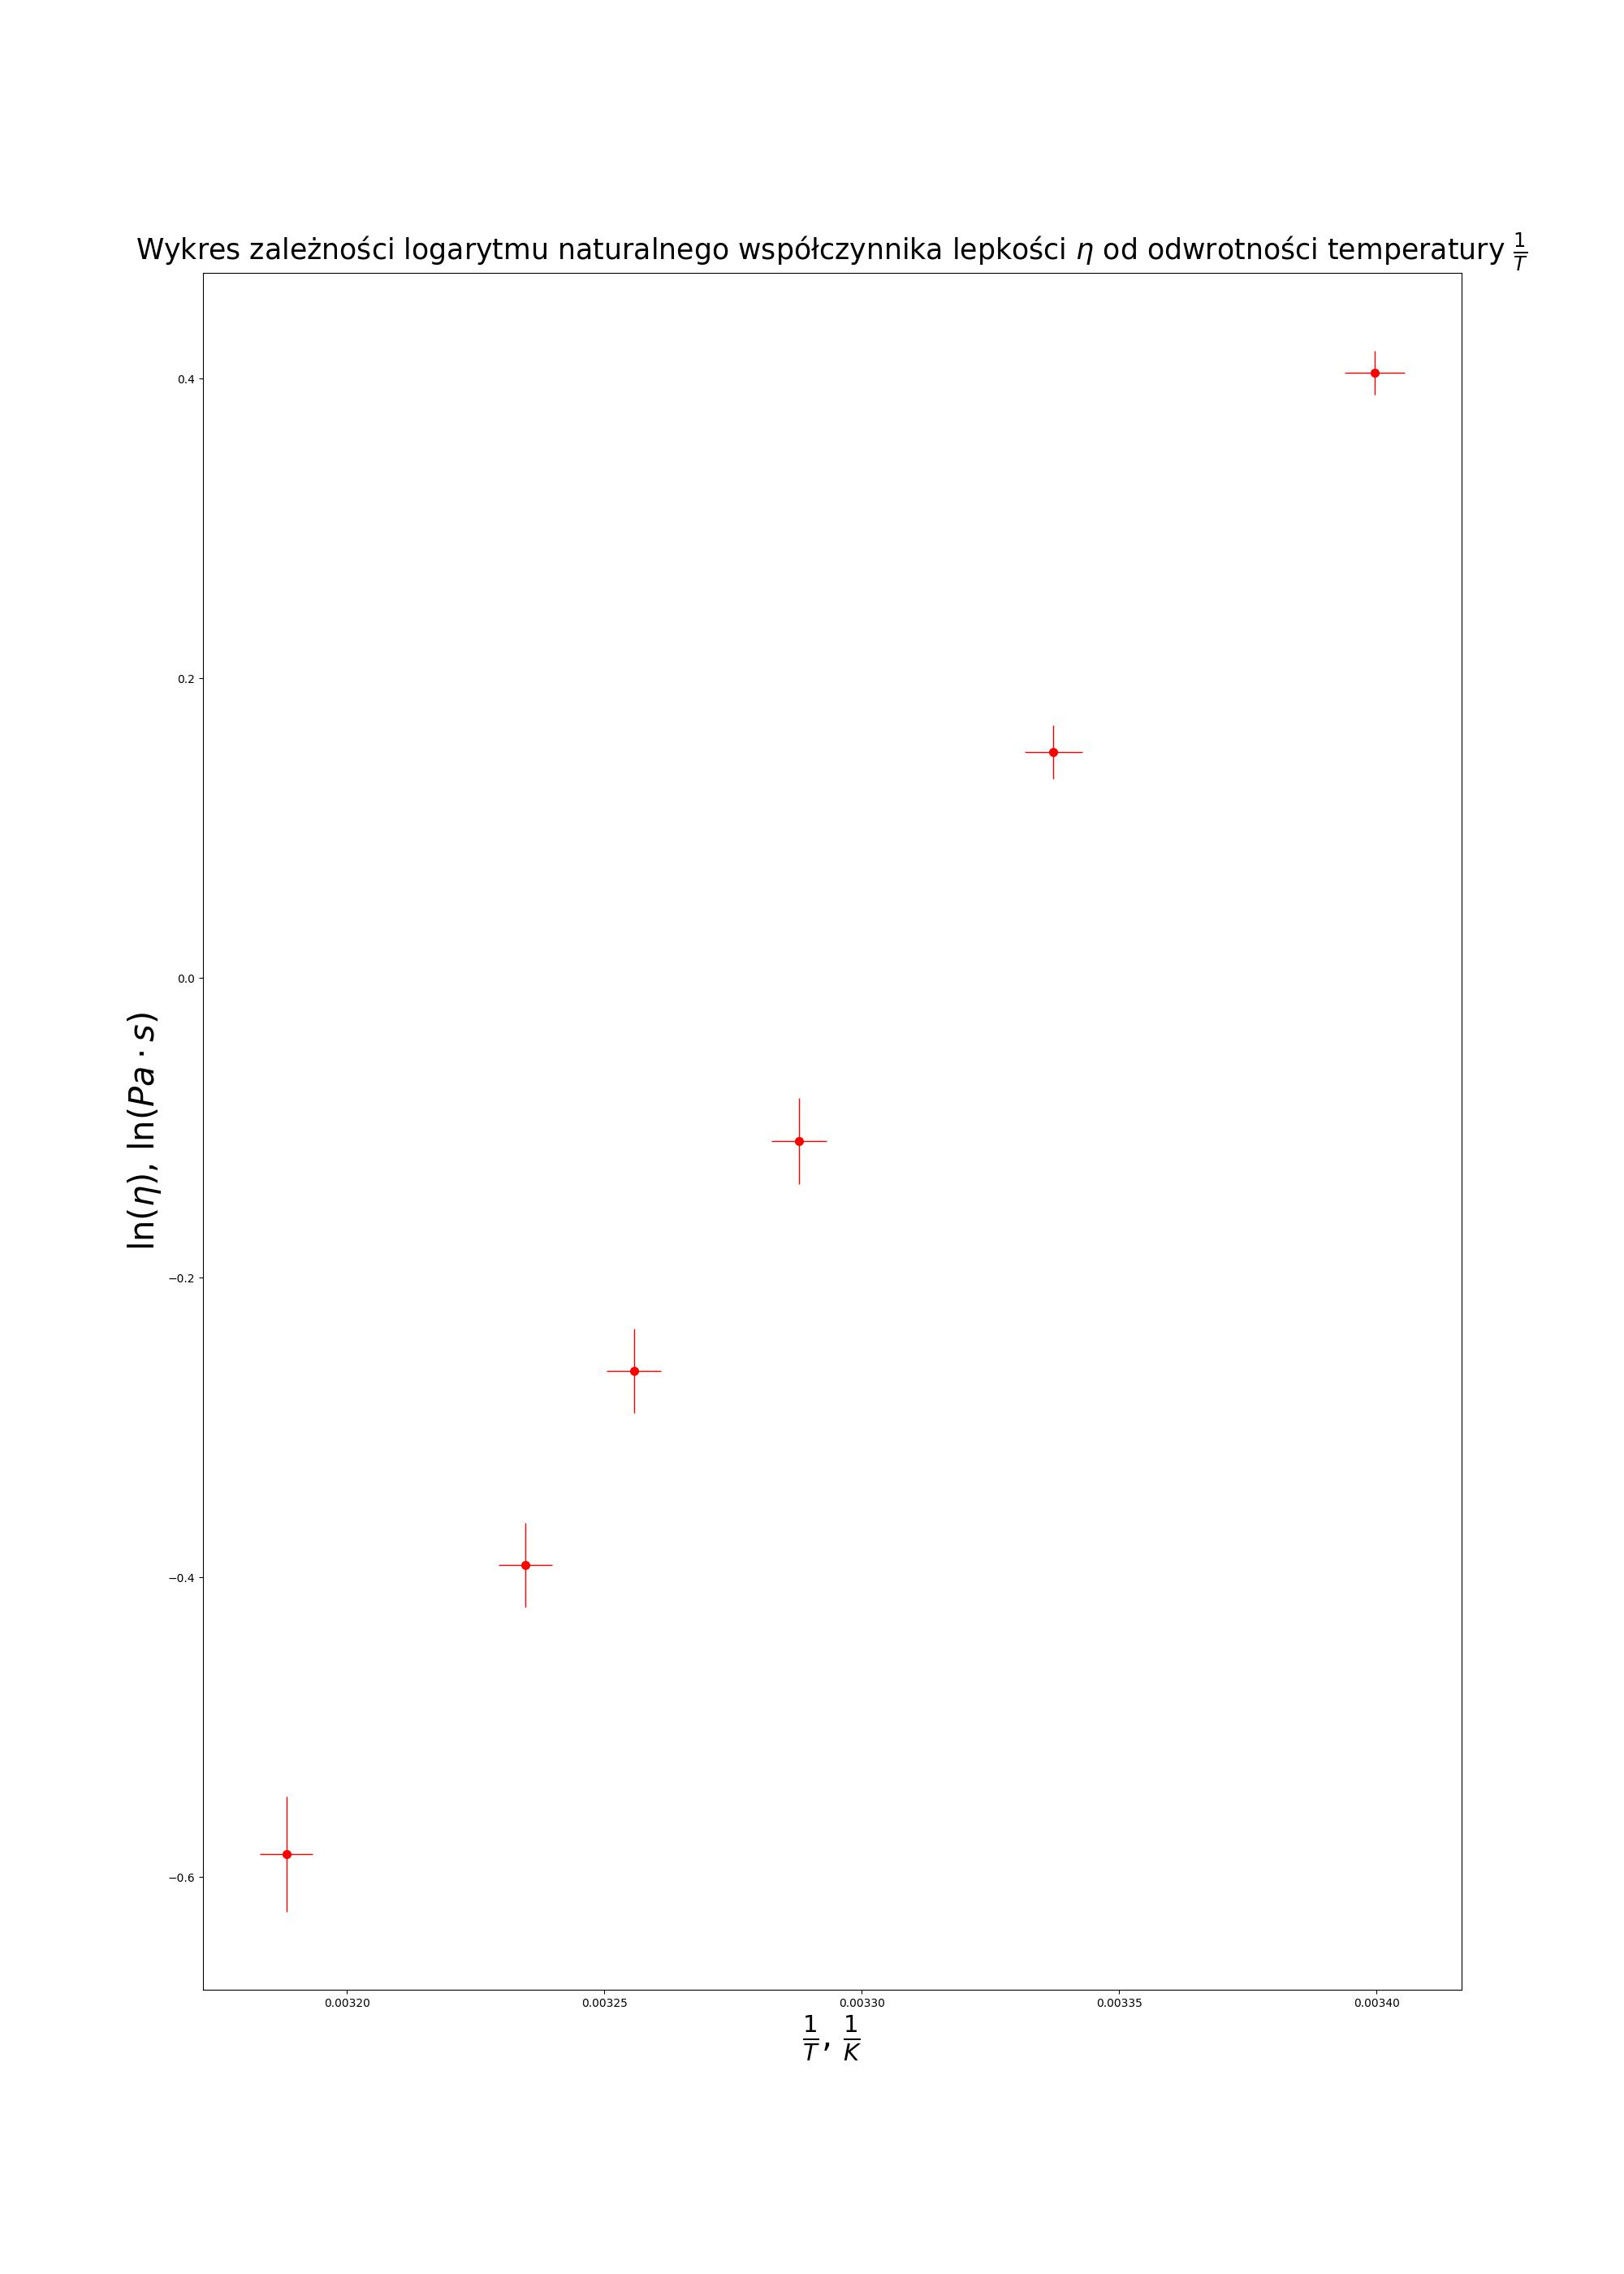
\includepdf{./img/wykres2.jpg}

\subsection*{Wyznaczenie metodą regresji liniowej współczynników funkcji $\eta(T)$
    wraz z niepewnościami.}

Aby policzyć współczynniki kierunkowe prostych i wyrazy wolne skorzystamy ze wzorów:

\begin{center}
    $a = \frac{nS_{xy} - S_xS_y}{nS_{xx}-S_x^2}$, $b =\frac{S_{xx}S_y-S_xS_{xy}}{nS_{xx}-S_x^2}$
\end{center}
Gdzie:
\begin{center}
    $S_x=\displaystyle\sum_{i=1}^{n}x_i$,
    $S_y=\displaystyle\sum_{i=1}^{n}y_i$,
    $S_{xx}=\displaystyle\sum_{i=1}^{n}x_i^2$,
    $S_{xy}=\displaystyle\sum_{i=1}^{n}x_i \cdot y_i$ \\
\end{center}
Do obliczenia niepewności skorzystamy ze wzorów:
\begin{center}
    $u(a) = \sqrt{\frac{n}{n-2} \cdot
            \frac{S_{\epsilon\epsilon}}{nS_{xx}-S_x^2}}$, $u(b) = \sqrt{\frac{1}{n-2} \cdot
        \frac{S_{xx}S_{\epsilon\epsilon}}{nS_{xx}-S_x^2}}$ \\
\end{center}
Gdzie:
\begin{center}
    $S_{\epsilon\epsilon}=\displaystyle\sum_{i=1}^{n}\epsilon_i^2$, dla $\epsilon_i = y_i - ax_i - b$
\end{center}
Po obliczeniach wartości współczynników są równe:

$a = -0.0494 \frac{Pa \cdot s}{^{\circ}C}$,

$b = 2.48$ Pa$\cdot$s. \\
Wartości niepewności współczynników prostej:

$u(a) = 0.0037 \frac{Pa \cdot s}{^{\circ}C}$,

$u(b) = 0.12$ Pa$\cdot$s. \\
Postać końcowa:

$a = -0.0494(37) \frac{Pa \cdot s}{^{\circ}C}$,

$b = 2.48(12)$ Pa$\cdot$s.

\subsection*{Obliczenie współczynników regresji $b=\ln(A)$ i $a= W/k$
    (wraz z niepewnościami) zależności opisującej \\
    temperaturową zależność współczynnika lepkości.}

Temperaturowa zależność współczynnika lepkości:
\begin{center}
    $ \eta(T) = Ae^{\frac{W}{kT}}$
\end{center}
Gdzie:

$k = 1.38 \cdot 10^{-23} \frac{J}{K}$ - stała Boltzmanna.

$W$ - energia aktywacji przepływu lepkiego. \\
Po przekształceniach otrzymujemy:
\begin{center}
    $ \ln(\eta(T)) = \ln(A) + \frac{W}{kT}$ \\
    $ \ln(\eta(T)) = \frac{a}{T} + b$ \\
    $ \ln(\eta(\frac{1}{T})) = aT + b$
\end{center}
Teraz możemy obliczyć współczynniki regresji funkcji
$f(\frac{1}{T}) = \ln(\eta)$, aby \\
wyliczyć $a$ i $b$.

$a$ = 4790 K$\cdot \ln$(Pa $\cdot$ s),

$b$ = -15.80 $\ln$(Pa $\cdot$ s). \\
Niepewności:

$u(a)$ = 120 K$\cdot \ln$(Pa $\cdot$ s),

$u(b)$ = 0.40 $\ln$(Pa $\cdot$ s). \\
Postać końcowa:

$a = 4790(120)$ K $\cdot \ln$(Pa $\cdot$ s),

$b = -15.80(40) \ln$(Pa $\cdot$ s).

\subsection*{Obliczenie energi aktywacji przepływu lepkiego $W$.}
Aby policzyć energie aktywacji przepływu lepkiego, skorzystamy ze wzoru:
\begin{center}
    $W = a \cdot k$
\end{center}
Po wstawieniu danych:
\begin{center}
    $W = 4790 \cdot 1.38 \cdot 10^{-23} = 6.61 \cdot 10^{-20} \frac{J}{mol}$.
\end{center}
Przeliczniki:
\begin{center}
    $1 \frac{J}{mol} = 1.66 \cdot 10^{-24}$ J. \\
    $1$ J $ = 6.24 \cdot 10^{18}$ eV.
\end{center}
Zapisanie wyniku w odpowiednich jednostkach:
\begin{center}
    $W = 6.61 \cdot 10^{-20} \frac{J}{mol} = 1.10 \cdot 10^{-43}$ J. \\
    $W = 1.10 \cdot 10^{-43}$ J $ = 6.84 \cdot 10^{-25}$ eV.
\end{center}

\subsection*{Obliczenie niepewności energi aktywacji przepływu \\
    lepkiego $W$ korzystając z prawa przenoszenia \\
    niepewności.}
Prawo przenoszenia niepewności dla $W$ ma postać:
\begin{center}
    $u(W) = \sqrt{[k \cdot u(a)]^2} = k \cdot u(a)$.
\end{center}
Po obliczeniach:
\begin{center}
    $u(W) = 1.70 \cdot 10^{-21} \frac{J}{mol}  = 2.8 \cdot 10^{-45}$ J. \\
    $u(W) = 2.82 \cdot 10^{-45}$ J $ = 1.8 \cdot 10^{-26}$ eV.
\end{center}

\subsection*{Zapisanie wyniku i niepewności w stosownym formacie w J i eV.}
Końcowa postać dla $W$ w J i eV: 
\begin{center}
    $W = 1.100(28) \cdot 10^{-43}$ J. \\
    $W = 6.84(18) \cdot 10^{-25}$ eV.
\end{center}

\subsection*{Wnioski.}
Na podstawie wykonanych obliczeń i wykresów, widać, że 
współczynnik lepkości cieczy $\eta$ zależy od temperatury cieczy;
im większa temperatura, tym współczynnik lepkości jest mniejszy, co
za tym idzie, kulka opada szybciej.

Niepewności pomiarowe wynikają z niedokładnego odczytu temperatury
na termometrze, niedokładnego zmierzenia czasu spowodowanego opóźnieniem
w czasie reakcji człowieka.
\end{document}
